\documentclass{article}

\usepackage{graphicx} %[pdftex] OR [dvips]
\usepackage{fullpage}
\usepackage{float}
\usepackage{titling}
\usepackage{hyperref}
\setlength{\droptitle}{-6em}

\newcommand{\ghcfile}[1]{\textsl{#1}}

\title{Implementing Backpack}

\begin{document}

\maketitle

The purpose of this document is to describe an implementation path
for Backpack~\cite{Kilpatrick:2014:BRH:2535838.2535884} in GHC\@.

We start off by outlining the current architecture of GHC, ghc-pkg and Cabal,
which constitute the existing packaging system.  We then state what our subgoals
are, since there are many similar sounding but different problems to solve.  Next,
we describe the ``probably correct'' implementation plan, and finish off with
some open design questions.  This is intended to be an evolving design document,
so please contribute!

\section{Current packaging architecture}

The overall architecture is described in Figure~\ref{fig:arch}.

\begin{figure}[H]
    \center{\scalebox{0.8}{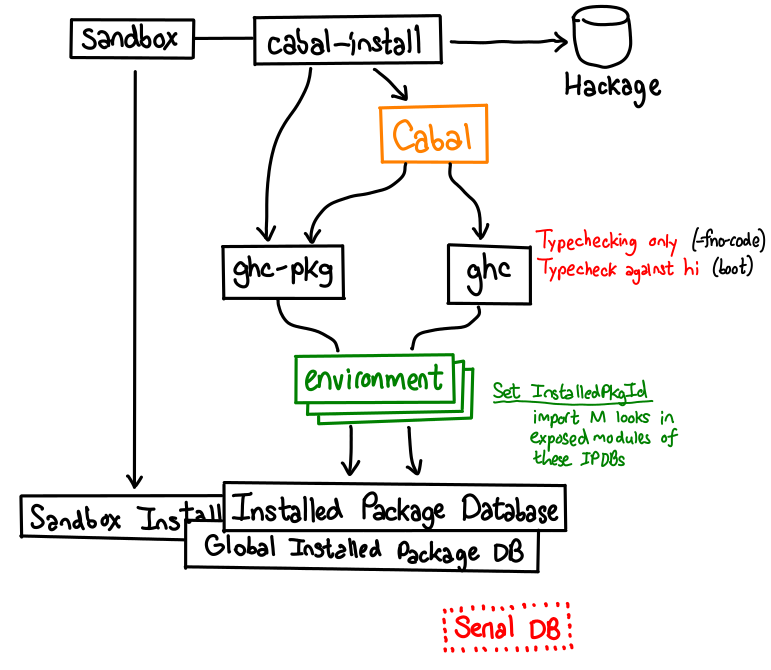
\includegraphics{arch.png}}}
\label{fig:arch}\caption{Architecture of GHC, ghc-pkg and Cabal. Green bits indicate additions from upcoming IHG work, red bits indicate additions from Backpack.  Orange indicates a Haskell library.}
\end{figure}

Here, arrows indicate dependencies from one component to another.  Color
coding is as follows: orange components are libaries, green components
are to be added with the IHG work, red components are to be added with
Backpack.  (Thus, black and orange can be considered the current)

\subsection{Installed package database}

Starting from the bottom, we have the \emph{installed package database}
(actually a collection of such databases), which stores information
about what packages have been installed are thus available to be
compiled against.  There is both a global database (for the system
administrator) and a local database (for end users), which can be
updated independently.  One way to think about the package database
is as a \emph{cache of object code}.  In principle, one could compile
any piece of code by repeatedly recompiling all of its dependencies;
the installed package database describes when this can be bypassed.

\begin{figure}[H]
    \center{\scalebox{0.8}{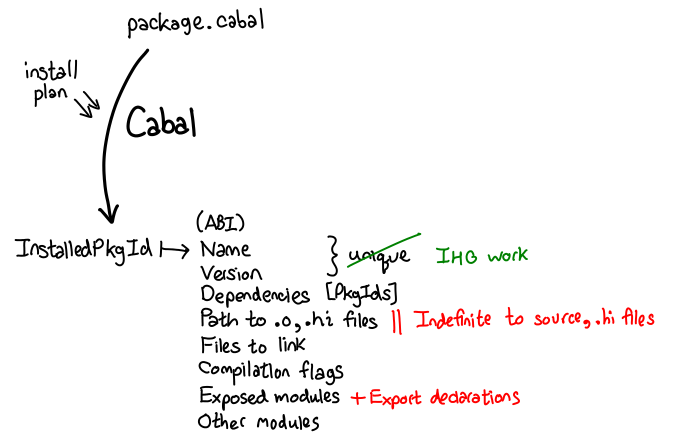
\includegraphics{pkgdb.png}}}
\label{fig:pkgdb}\caption{Anatomy of a package database.}
\end{figure}

In Figure~\ref{fig:pkgdb}, we show the structure of a package database.
The installed package are created from a Cabal file through the process
of dependency resolution and compilation.  In database terms, the primary key
of a package database is the InstalledPackageId
(Figure~\ref{fig:current-pkgid}).  This ID uniquely identifies an
instance of an installed package.  The PackageId omits the ABI hash and
is used to qualify linker exported symbols: the current value of this
parameter is communicated to GHC using the \verb|-package-id| flag.

In principle, packages with different PackageIds should be linkable
together in the same compiled program, whereas packages with the same
PackageId are not (even if they have different InstalledPackageIds).  In
practice, GHC is currently only able to select one version of a package,
as it clears out all old versions of the package in
\ghcfile{compiler/main/Package.lhs}:applyPackageFlag.

\begin{figure}
    \center{\begin{tabular}{r l}
        PackageId & package name, package version \\
        InstalledPackageId & PackageId, ABI hash \\
    \end{tabular}}
\label{fig:current-pkgid}\caption{Current structure of package identifiers.}
\end{figure}

The database entry itself contains the information from the installed package ID,
as well as information such as what dependencies it was linked against, where
its compiled code and interface files live, its compilation flags, what modules
it exposes, etc.  Much of this information is only relevant to Cabal; GHC
uses a subset of the information in the package database.

\subsection{GHC}

The two programs which access the package database directly are GHC
proper (for compilation) and ghc-pkg (which is a general purpose
command line tool for manipulating the database.)  GHC relies on
the package database in the following ways:

\begin{itemize}
    \item It imports the local and global package databases into
        its runtime database, and applies modifications to the exposed
        and trusted status of the entries via the flags \verb|-package|
        and others (\ghcfile{compiler/main/Packages.lhs}).  The internal
        package state can be seen at \verb|-v4| or higher.
    \item It uses this package database to find the location of module
        interfaces when it attempts to load the module info of an external
        module (\ghcfile{compiler/iface/LoadIface.hs}).
\end{itemize}

GHC itself performs a type checking phase, which generates an interface
file representing the module (so that later invocations of GHC can load the type
of a module), and then after compilation projects object files and linked archives
for programs to use.

\paragraph{Original names} Original names are an important design pattern
in GHC\@.
Sometimes, a name can be exposed in an hi file even if its module
wasn't exposed. Here is an example (compiled in package R):

\begin{verbatim}
module X where
    import Internal (f)
    g = f

module Internal where
    import Internal.Total (f)
\end{verbatim}

Then in X.hi:

\begin{verbatim}
g = <R.id, Internal.Total, f> (this is the original name)
\end{verbatim}

(The reason we refer to the package as R.id is because it's the
full package ID, and not just R).

\subsection{hs-boot}

\verb|hs-boot| is a special mechanism used to support recursive linking
of modules within a package, today.  Suppose I have a recursive module
dependency between modules and A and B. I break one of\ldots

(ToDo: describe how hs-boot mechanism works)

\subsection{Cabal}

Cabal is the build system for GHC, we can think of it as parsing a Cabal
file describing a package, and then making (possibly multiple)
invocations to GHC to perform the appropriate compilation.  What
information does Cabal pass onto GHC\@?  One can get an idea for this by
looking at a prototypical command line that Cabal invokes GHC with:

\begin{verbatim}
ghc --make
    -package-name myapp-0.1
    -hide-all-packages
    -package-id containers-0.9-ABCD
    Module1 Module2
\end{verbatim}

There are a few things going on here.  First, Cabal has to tell GHC
what the name of the package it's compiling (otherwise, GHC can't appropriately
generate symbols that other code referring to this package might generate).
There are also a number of commands which configure its in-memory view of
the package database (GHC's view of the package database may not directly
correspond to what is on disk).  There's also an optimization here: in principle,
GHC can compile each module one-by-one, but instead we use the \verb|--make| flag
because this allows GHC to reuse some data structures, resulting in a nontrivial
speedup.

(ToDo: describe cabal-install/sandbox)

\section{Goals}

There are actually a number of different goals we have for modifying the
packaging system, some of which are subsets of the Backpack system.

\begin{itemize}
    \item As a prerequisite, support multiple instances of containers-2.9 \emph{in the
        package database}.  These instances may be compiled against
        different dependencies, have the same dependencies but different
        source files (as when a package is being developed), or be
        compiled with different options.  It is less important to allow
        these instances to be linkable together.\footnote{Actually, I think
        this is completely orthogonal to Backpack, since we are going to treat
        dependencies as part of the package ID, so they would be considered
        separate entries in the package database anyway.}

    \item Support typechecking a library against a module interface
        as opposed to an actual implementation.  This includes not
        only support proper, but also toolchain support for generating
        and keeping interface files up-to-date, and taking advantage
        of this discipline to augment Cabal package dependency resolution
        with proper signature packages. %  See Section~\ref{sec:signature-packages} for more details.

    \item Support compiling the aforementioned libraries with actual implementations.
        It is \emph{not} a goal to be able to compile a library while only
        partially providing dependencies, and it is low priority to support
        mutually recursive implementations of these implementations.
\end{itemize}

A lower priority goal is to actually allow multiple instances of
containers-2.9 to be linked together in the same executable
program.\footnote{In particular, this requires changes to how linker
symbols are assigned. However, this feature is important to
implement a number of Backpack features.}

A \emph{non-goal} is to allow users to upgrade upstream libraries
without recompiling downstream. This is an ABI concern and we're not
going to worry about it.

\section{Aside: Recent IHG work}\label{sec:ihg}

The IHG project has allocated some funds to relax the package instance
constraint in the package database, so that multiple instances can be
stored, but now the user of GHC must explicitly list package-IDs to be
linked against.  In the far future, it would be expected that tools like
Cabal automatically handle instance selection among a large number of
instances, but this is subtle and so this work is only to do some
foundational work, allowing a package database to optionally relax the
unique package-version requirement, and utilize environment files to
select which packages should be used.  See Duncan's email for more
details on the proposal.

To implement this:

\begin{enumerate}

    \item Remove the ``removal step'' when registering a package (with a flag)

    \item Check \ghcfile{compiler/main/Packages.lhs}:mkPackagesState to look out for shadowing
      within a database. We believe it already does the right thing, since
      we already need to handle shadowing between the local and global database.

\end{enumerate}

Once these changes are implemented, we can program multiple instances by
using \verb|-hide-all-packages -package-id ...|, even if there is no
high-level tool support.

Actually, this concern is orthogonal to the purposes of Backpack, if
we redefine PackageId appropriately.

\paragraph{The ABI hash} Currently, InstalledPackageId
is constructed of a package, version and ABI hash
(generateRegistrationInfo in
\ghcfile{libraries/Cabal/Cabal/Distribution/Simple/Register.hs}).  The
use of an ABI hash is a bit of GHC-specific hack introduced in 2009,
intended to make sure these installed package IDs are unique.  While
this is quite clever, using the ABI is actually a bit inflexible, as one
might reasonably want to have multiple copies of a package with the same
ABI but different source code changes.\footnote{In practice, our ABIs
are so unstable that it doesn't really matter.}

In Figure~\ref{fig:proposed-pkgid}, there is an alternate logical
representation of InstalledPackageId which attempts to extricate the
notion of ABI compatibility from what actually might uniquely identify a
package beyond its PackageId.  We imagine these components to be:

\begin{itemize}
    \item A hash of the source code (so one can register different
        in-development versions without having to bump the version
        number);
    \item Compilation way (profiling? dynamic?)
    \item Compilation flags (such as compilation way, optimization,
        profiling settings)\footnote{This is a little undefined on a package bases, because in principle the flags could be varied on a per-file basis. More likely this will be approximated against the relevant fields in the Cabal file as well as arguments passed to Cabal.};
\end{itemize}

A historical note: in the 2012 GSoC project to allow multiple instances
of a package to be installed at the same time, use of \emph{random
numbers} was used to workaround the inability to get an ABI early
enough.  We are not using this plan.

\section{Infrastructural improvements}

There are some infrastructural improvements that must be made before
Backpack proper can be implemented.  These additions are described in
red in the architectural diagrams.  The current structure of this
section is to describe the additions bottom up.

\subsection{Concrete physical identity = PackageId + Module name + Module dependencies}\label{sec:ipi}

\begin{figure}
    \center{\begin{tabular}{r l}
            PackageId & hash of ``package name, package version, dependency resolution, \emph{module} environment'' \\
        InstalledPackageId & hash of ``PackageId, source code, way, compiler flags'' \\
    \end{tabular}}
\label{fig:proposed-pkgid}\caption{Proposed new structure of package identifiers.}
\end{figure}

In Backpack, there needs to be some mechanism for assigning
\emph{physical module identities} to modules, which are essential for
typechecking Backpack packages, since they let us tell if two types are
equal or not.

In GHC, our method of testing whether or not two types are equal is by
comparing their original names, which is a tuple of a PackageId and the
module name (summarized in Figure~\ref{fig:current-pkgid}).  If it looks
like a duck and quacks like a duck, it is a duck: we might reasonable
imagine that \emph{concrete physical identity = PackageId and module
name}.  But is this sufficient to represent Backpack's physical module
identities?

If we look at how physical module identities are allocated in Paper Backpack,
we can see that each module corresponds to an identity constructor (in
Backpack this is the package name, some representation of the module
source, and a disambiguating integer if module source is duplicated)
\emph{as well as} physical module identities which were applied to
this constructor.  The current PackageId + Module name scheme adequately encodes
the constructor (in particular, a single package can't have multiple modules
with the same name), but it does not encode the \emph{module} dependencies.
We have to add these to our original names.  There are three ways we can do
this:

\begin{enumerate}
    \item Augment original names to have a third component.  This is less than ideal because it requires pervasive changes to all parts of the compiler.
    \item Augment the module name to record module dependency information.  This is a bit of an odd place to put the information, because our module names correspond quite concretely to the actual source file a user wrote some source in.
    \item Augment the PackageId to record module dependency information.  For now, this is the regime we will use; however, see Section~\ref{sec:flatten} for why the issue is more subtle.
\end{enumerate}

(XXX Figure~\ref{fig:proposed-pkgid} is out of date now.)

And now, the complications\ldots

\paragraph{Relaxing package selection restrictions}  As mentioned
previously, GHC is unable to select multiple packages with the same
package name (but different PackageIds).  This restriction needs to be
lifted.  For backwards compatibility reasons, it's probably better to
not overload \verb|-package-id| but add a new flag, maybe \verb|-force-package-id|;
we also need to disable the old version masking behavior.  This is orthogonal
to the IHG work, which wants to allow multiple \emph{InstalledPackageIds} in the
\emph{database} (here, we want to allow multiple \emph{PackageIds} in \emph{compiled code}).

\paragraph{Linker symbols} As we increase the amount of information in
PackageId, it's important to be careful about the length of these IDs,
as they are used for exported linker symbols (e.g.
\verb|base_TextziReadziLex_zdwvalDig_info|).  Very long symbol names
hurt compile and link time, object file sizes, GHCi startup time,
dynamic linking, and make gdb hard to use.  As such, the current plan is
to do away with full package names and versions, and instead use just a
base-62 encoded hash, perhaps with the first four characters of the package
name for user-friendliness.

Edward: I'm still partial to a short hash of the dependency bits (or
even Simon's registry of short strings to dependency trees), and keeping
everything else the same.

\paragraph{Wired-in names} One annoying thing to remember is that GHC
has wired-in names, which refer to packages without any version.  Now
these wired names also have to accomodate dependency trees. A
suggested approach is to have a fixed table from these wired names to
package IDs; alternately we can use something like the special \verb|inplace|
version number.

\paragraph{Version numbers}  The interaction of Backpack's package polymorphism
(the ability to mixin different implementations to holes) and Cabal's dependency
resolution mechanism (which permits a name libfoo to be resolved to a specific
version libfoo-0.1) can be subtle: there are in fact \emph{two} levels of
indirection going on here.

The simplest way to think about the distinction is as follows.  When I write
a Backpack package which does \verb|include foobar|, I have not actually
written a Paper Backpack package.  Instead, I have written a \emph{pre-package},
which Cabal's dependency solver then takes and rewrites all package references
into versioned references \verb|include foobar-0.1|, which now corresponds to
a Paper Backpack package.  For example, this is a pre-package:

\begin{verbatim}
package foo where
    include bar
\end{verbatim}

and this is a Paper Backpack package:

\begin{verbatim}
package foo-0.3(bar-0.1) where
    include bar-0.1(baz-0.2)
\end{verbatim}

Notably, we must \emph{rename} the package to include information about
how we resolved all of the inner package references, and if these inner
package references had dependencies, those must be included too!  In
effect, the \emph{dependency resolution} must be encoded into the package ID,
along with the existing Backpack \emph{physical identity regular tree}.
Phew!

\paragraph{Free variables (or, what is a non-concrete physical
identity?)} Physical identities in their full generality are permitted
to have free variables, which represent holes.  Handling this is a
tricky question, and we defer it to Section~\ref{sec:typechecking-indefinite}, when
we talk about packages with holes.

\subsection{Flatten the package database}\label{sec:flatten}

In the previous section, I implied that the \emph{module} dependencies
could be recorded with the \emph{package} ID\@.  Type error? Yes!

In the old world order, we think of dependencies as being associated with
packages as a whole.  However, Paper Backpack specifies dependency tracking
at the \emph{module} level, which means that different compilations of
an indefinite package may result in modules which should be identified.
Here is a Backpack package which demonstrates the issue:

\begin{verbatim}
package a where
    P :: ...
    Q :: [ x :: Int ]
    A = [ import P; ... ]
    B = [ import Q; ... ]
package p where
    P = [ ... ]
package x where
    include p
    Q = [ x = 0 ]
    include a
package y where
    include p
    Q = [ x = 1 ]
    include a
\end{verbatim}

Here, we have a package \verb|a| which probably should have been defined as
two separate packages (since \verb|A| only relies on \verb|P| and \verb|B|
only relies on \verb|Q|), but the functionality has been glommed together.
Then, the downstream packages \verb|x| and \verb|y| fill in the holes using the
same implementation of \verb|P|, but differing implementations of \verb|Q|.
(For more explanation about how we would go about compiling this set of
packages, please see Section~\ref{sec:compiling-definite}.)

Is module \verb|A| from package \verb|x| the same as module \verb|A|
from package \verb|y|?  In Paper Backpack, the answer is yes.
However, presently, the installed package database acts as a cache at the \emph{package}
level; code is only shared if it comes from the same package.  Can we share
packages \verb|x| and \verb|y|? No!
\verb|x:B| is \emph{not} the same module as \verb|y:B| (they are using differing
versions of \verb|Q|).  The upshot is that we are in an awkward position,
where package \verb|a| contains some modules which must be distinct, and other
modules which must be unified over several installs.

The theory, thus, demands that we flatten the package database, so that
we no longer insist that all compiled code that is produced when a
package is installed live together in a single directory: instead,
\emph{the installed package database is a directory of physical module
identities to objects/interfaces}.  Installed packages are represented
as (possibly overlapping) sets over this store of modules.

\paragraph{Do we really care about this use case?}  Scott gave me one
good argument why this is a nice feature to have: it permits users to
modularize third-party packages which were not packaged with modularity
in mind, but happen to be modular.  For example, when libraries ship
with test-cases, they currently have to split these test-cases to separate
packages, so as to not introduce spurious dependencies with various
test frameworks, which the user may not have or care about.  If dependencies
are done on a per-module basis, as long as the user doesn't import a test
module, they never gain the extra dependency.  Another situation is when
a library also happens to have a helper utility module which doesn't have
any of the dependencies of the primary library.

One could argue that people already understand it is good practice to
separate such cases into separate packages, and there is no pressing
need to allow for sloppy habits.  The counterargument, however, is that
you are often not in control of these third-party libraries, and the
more control in the end-user's hands, the better.

\paragraph{Operating system linking}  When the package database is flattened
into a collection of modules, it becomes less clear how to generate library
files corresponding to a package.  One possibility is to simply take the
set of files corresponding to a package and wrap it up into a library.
If an end-user links against two libraries which include the same object file,
the linker needs to suppress the symbols associated with one of the instances
of the object file (it's identical, right?)\footnote{It may not actually be
possible to do this in the static linking case: one must refer to the actual object
files}.

If your modules are truly applicative, this might even work OK\@.  However, you will
be a sad panda if there is any unsafe, mutable global state in the shared
object (since the object files will each get separate data segments for this
global state): a generative semantics.\footnote{Even if we did get this right,
which would be possible when statically linking these modules together, the
interaction could still be surprising: Backpack can remodularize modules, but
it can't remodularize values inside a module, so if a module has a dependency
but some global state in the module doesn't, the resulting behavior can be
surprising.  Perhaps the moral of the story really is, ``Don't do side effects
in an applicative module system! No really!''} \\

\subsection{Alternatives to flattening package DB}
Flattening can be seen as one of four different representations of packages
at the OS/library level. While it promotes maximal sharing of identical
modules, it is perhaps too fine-grained for most purposes.
\emph{ToDo: Describe the alternatives.}

\paragraph{Package slicing} Instead of changing the package database,
we automatically
slice a single package into multiple packages, so that the sliced
packages have dependencies which accurately reflect their constitutent
modules.  For a well modularized package, the slicing operation should
be a no-op.  This would also be useful in some other situations (see the
\verb|-module-env| discussion in Section~\ref{sec:compiling-definite}).
In fact, which slice a module should be placed in can be automatically
calculated by taking the package name with the regular tree
associated with the module (Section~\ref{sec:ipi}).

A minor downside of package slicing is in a dynamically linked environment,
we pay a performance cost when we have to jump from one dynamic library
to another, and slicing could introduce are large number of separate
dynamic libraries which need to be switched between each other.

Edward likes this proposal.

\paragraph{Changing Backpack to disallow fine-grained dependencies}

Another perspective is that we fell into a trap when we decided that
dependencies should be calculated per-module.  What if, instead, we
expanded the dependency of each module to cover \emph{all signatures}
in the package?  Then the dependency tree would always be the same and
the package would be shared only if all holes were precisely the same.
Our motivating example, then, would fail to witness sharing.

This might be the simplest thing to do, but it is a change in the
Backpack semantics, and rules out modularization without splitting a package
into multiple packages.  Maybe Scott can give other reasons why this
would not be so good.  SPJ is quite keen on this plan.

\subsection{Exposed modules should allow external modules}\label{sec:reexport}

In Backpack, the definition of a package consists of a logical context,
which maps logical module names to physical module names.  These do not
necessarily coincide, since some physical modules may have been defined
in other packages and mixed into this package.  This mapping specifies
what modules other packages including this package can access.
However, in the current installed package database, we have exposed-modules which
specify what modules are accessible, but we assume that the current
package is responsible for providing these modules.

To implement Backpack, we have to extend this exposed-modules (``Export declarations''
on Figure~\ref{fig:pkgdb}).  Rather
than a list of logical module names, we provide a new list of tuples:
the exported logical module name and original physical module name (this
is in two parts: the InstalledPackageId and the original module name).
For example, an traditional module export is simply (Name, my-pkg-id, Name);
a renamed module is (NewName, my-pkg-id, OldName), and an external module
is (Name, external-pkg-id, Name).

As an example:

\begin{verbatim}
package P where
    M = ...
    N = ...
package Q (M, R, T)
    include P (N -> R)
    T = ...
\end{verbatim}

And now if we look at Q\@:

\begin{verbatim}
exposed-modules:
        <M, P.id, M>
        <R, P.id, N>
        <T, Q.id, T>
\end{verbatim}

When we compile Q, and the interface file gets generated, we have
to generate identifiers for each of the exposed modules.  These should
be calculated to directly refer to the ``original name'' of each them;
so for example M and R point directly to package P, but they also
include the original name they had in the original definition.

\paragraph{Error messages}  When it is possible for multiple physical
entities to have the same ``user-friendly'' name, this can result in a
very confusing situation if both entities have to be referred to in the
same message.  This is especially true when renaming is in place:
you not only want to print out the name in scope, but probably some indication
of what the original name is.  In short, when it comes to error messages, tread with care!

\section{Shapeless Backpack}\label{sec:simplifying-backpack}

Backpack as currently defined always requires a \emph{shaping} pass,
which calculates the shapes of all modules defined in a package.
The shaping pass is critical to the solution of the double-vision problem
in recursive module linking, but it also presents a number of unpalatable
implementation problems:

\begin{itemize}

    \item \emph{Shaping is a lot of work.} A module shape specifies the
        providence of all data types and identifiers defined by a
        module. To calculate this, we must preprocess and parse all
        modules, even before we do the type-checking pass.  (Fortunately,
        shaping doesn't require a full parse of a module, only enough
        to get identifiers, which makes it a slightly more expensive
        version of \verb|ghc -M|.)

    \item \emph{Shaping must be done upfront.} In the current Backpack
        design, all shapes must be computed before any typechecking can
        occur.  While performing the shaping pass upfront is necessary
        in order to solve the double vision problem (where a module
        identity may be influenced by later definitions), it means
        that GHC must first do a shaping pass, and then revisit every module and
        compile them proper.  Nor is it (easily) possible to skip the
        shaping pass when it is unnecessary, as one might expect to be
        the case in the absence of mutual recursion.  Shaping is not
        a ``pay as you go'' language feature.

    \item \emph{GHC can't compile all programs shaping accepts.}  Shaping
        accepts programs that GHC, with its current hs-boot mechanism, cannot
        compile.  In particular, GHC requires that any data type or function
        in a signature actually be \emph{defined} in the module corresponding
        to that file (i.e., an original name can be assigned to these entities
        immediately.)  Shaping permits unrestricted exports to implement
        modules; this shows up in the formalism as $\beta$ module variables.

    \item \emph{Shaping encourages inefficient program organization.}
        Shaping is designed to enable mutually recursive modules, but as
        currently implemented, mutual recursion is less efficient than
        code without recursive dependencies. Programmers should avoid
        this code organization, except when it is absolutely necessary.

    \item \emph{GHC is architecturally ill-suited for directly
        implementing shaping.}  Shaping implies that GHC's internal
        concept of an ``original name'' be extended to accommodate
        module variables.  This is an extremely invasive change to all
        aspects of GHC, since the original names assumption is baked
        quite deeply into the compiler.  Plausible implementations of
        shaping requires all these variables to be skolemized outside
        of GHC\@.

\end{itemize}

To be clear, the shaping pass is fundamentally necessary for some
Backpack packages.  Here is the example which convinced Simon:

\begin{verbatim}
package p where
    A :: [data T; f :: T -> T]
    B = [export T(MkT), h; import A(f); data T = MkT; h x = f MkT]
    A = [export T(MkT), f, h; import B; f MkT = MkT]
\end{verbatim}

The key to this example is that B \emph{may or may not typecheck} depending
on the definition of A. Because A reexports B's definition T, B will
typecheck; but if A defined T on its own, B would not typecheck.  Thus,
we \emph{cannot} typecheck B until we have done some analysis of A (the
shaping analysis!)

Thus, it is beneficial (from an optimization point of view) to
consider a subset of Backpack for which shaping is not necessary.
Here is a programming discipline which does just that, which we will call the \textbf{linking restriction}: \emph{Module implementations must be declared before
signatures.}  Formally, this restriction modifies the rule for merging
polarized module shapes ($\widetilde{\tau}_1^{m_1} \oplus \widetilde{\tau}_2^{m_2}$) so that
$\widetilde{\tau}_1^- \oplus \widetilde{\tau}_2^+$ is always undefined.\footnote{This seemed to be the crispest way of defining the restriction, although this means an error happens a bit later than I'd like it to: I'd prefer if we errored while merging logical contexts, but we don't know what is a hole at that point.}

Here is an example of the linking restriction. Consider these two packages:

\begin{verbatim}
package random where
    System.Random = [ ... ].hs

package monte-carlo where
    System.Random :: ...
    System.MonteCarlo = [ ... ].hs
\end{verbatim}

Here, random is a definite package which may have been compiled ahead
of time; monte-carlo is an indefinite package with a dependency
on any package which provides \verb|System.Random|.

Now, to link these two applications together, only one ordering
is permissible:

\begin{verbatim}
package myapp where
    include random
    include monte-carlo
\end{verbatim}

If myapp wants to provide its own random implementation, it can do so:

\begin{verbatim}
package myapp2 where
    System.Random = [ ... ].hs
    include monte-carlo
\end{verbatim}

In both cases, all of \verb|monte-carlo|'s holes have been filled in by the time
it is included.  The alternate ordering is not allowed.

Why does this discipline prevent mutually recursive modules?  Intuitively,
a hole is the mechanism by which we can refer to an implementation
before it is defined; otherwise, we can only refer to definitions which
preceed our definition. If there are never any holes \emph{which get filled},
implementation links can only go backwards, ruling out circularity.

It's easy to see how mutual recursion can occur if we break this discipline:

\begin{verbatim}
package myapp2 where
    include monte-carlo
    System.Random = [ import System.MonteCarlo ].hs
\end{verbatim}

\subsection{Typechecking of definite modules without shaping}

If we are not carrying out a shaping pass, we need to be able to calculate
$\widetilde{\Xi}_{\mathsf{pkg}}$ on the fly.  In the case that we are
compiling a package---there will be no holes in the final package---we
can show that shaping is unnecessary quite easily, since with the
linking restriction, everything is definite from the get-go.

Observe the following invariant: at any given step of the module
bindings, the physical context $\widetilde{\Phi}$ contains no
holes.  We can thus conclude that there are no module variables in any
type shapes.  As the only time a previously calculated package shape can
change is due to unification, the incrementally computed shape is in
fact the true one.

As far as the implementation is concerned, we never have to worry
about handling module variables; we only need to do extra typechecks
against (renamed) interface files.

\subsection{Compilation of definite modules}\label{sec:compiling-definite}

Of course, we still have to compile the code, and this includes any
subpackages which we have mixed in the dependencies to make them fully
definite.  Let's take the following set of packages as an example:

\begin{verbatim}
package pkg-a where
    A = ...
    B = ... -- this code is ignored
package pgk-b where -- indefinite package
    A :: ...
    B = [ import A; ... ]
package pkg-c where
    include pkg-a (A)
    include pkg-b
    C = [ import B; ... ]
\end{verbatim}

With the linking invariant, we can simply walk the Backpack package ``tree'',
compiling each of its dependencies.  Let's walk through it explicitly.\footnote{To simplify matters, we assume that there is only one instance of any
PackageId in the database, so we omit the unique-ifying hashes from the
ghc-pkg registration commands; we ignore the existence of version numbers
and Cabal's dependency solver; finally, we do the compilation in
one-shot mode, even though Cabal in practice will use the Make mode.}

First, we have to build \verb|pkg-a|.  This package has no dependencies
of any kind, so compiling is much like compiling ordinary Haskell.  If
it was already installed in the database, we wouldn't even bother compiling it.

\begin{verbatim}
ADEPS =    # empty!
ghc -c A.hs -package-name pkg-a-ADEPS
ghc -c B.hs -package-name pkg-a-ADEPS
# install and register pkg-a-ADEPS
\end{verbatim}

Next, we have to build \verb|pkg-b|.  This package has a hole \verb|A|,
intuitively, it depends on package A.  This is done in two steps:
first we check if the signature given for the hole matches up with the
actual implementation provided, and then we build the module properly.

\begin{verbatim}
BDEPS = "A -> pkg-a-ADEPS:A"
# This doesn't actually create an hi-boot file
ghc -c A.hs-boot -package-name pkg-b-BDEPS -module-env BDEPS
ghc -c B.hs      -package-name pkg-b-BDEPS -module-env BDEPS
# install and register pkg-b-BDEPS
\end{verbatim}

Notably, these commands diverge slightly from the traditional compilation process.
Traditionally, we would specify the flags
\verb|-hide-all-packages| \verb|-package-id package-a-ADEPS| in order to
let GHC know that it should look at this package to find modules,
including \verb|A|.  However, if we did this here, we would also pull in
module B, which is incorrect, as this module was thinned out in the parent
package description.  Conceptually, this package is being compiled in the
context of some module environment \verb|BDEPS| (a logical context, in Backpack lingo)
which maps modules to original names and is utilized by the module finder to
lookup the import in \verb|B.hs|.

Finally, we created all of the necessary subpackages, and we can compile
our package proper.

\begin{verbatim}
CDEPS =         # empty!!
ghc -c C.hs -package-name pkg-c-CDEPS -hide-all-packages \
    -package pkg-a-ADEPS -hide-module B \
    -package pkg-b-BDEPS
# install and register package pkg-c-CDEPS
\end{verbatim}

This mostly resembles traditional compilation, but there are a few
interesting things to note.  First, GHC needs to know about thinning/renaming
in the package description (here, it's transmitted using the \verb|-hide-module|
command, intended to apply to the most recent package definition).\footnote{Concrete
command line syntax is, of course, up for discussion.}  Second, even though C
``depends'' on subpackages, these do not show in its package-name identifier,
e.g. CDEPS\@.  This is because this package \emph{chose} the values of ADEPS and BDEPS
explicitly (by including the packages in this particular order), so there are no
degrees of freedom.\footnote{In the presence of a Cabal-style dependency solver
which associates a-0.1 with a concrete identifier a, these choices need to be
recorded in the package ID.}  Finally, in principle, we could have also used
the \verb|-module-env| flag to communicate how to lookup the B import (notice
that the \verb|-package pkg-a-ADEPS| argument is a bit useless because we
never end up using the import.)  I will talk a little more about the tradeoffs
shortly.

Overall, there are a few important things to notice about this architecture.
First, because the \verb|pkg-b-BDEPS| product is installed, if in another package
build we instantiate the indefinite module B with exactly the same \verb|pkg-a|
implementation, we can skip the compilation process and reuse the version.
This is because the calculated \verb|BDEPS| will be the same, and thus the package
IDs will be the same.

XXX ToDo: actually write down pseudocode algorithm for this

\paragraph{Module environment or package flags?}  In the previous
section, I presented two ways by which one can tweak the behavior of
GHC's module finder, which is responsible for resolving \verb|import B|
into an actual physical module.  The first, \verb|-module-env| is to
explicitly describe a full mapping from module names to original names;
the second, \verb|-package| with \verb|-hide-module| and
\verb|-rename-module|, is to load packages as before but apply
thinning/renaming as necessary.

In general, it seems that using \verb|-package| is desirable, because its
input size is smaller. (If a package exports 200 modules, we would be obligated
to list all of them in a module environment.)  However, a tricky situation
occurs when some of these modules come from a parent package:

\begin{verbatim}
package myapp2 where
    System.Random = [ ... ].hs
    include monte-carlo
    App = [ ... ].hs
\end{verbatim}

Here, monte-carlo depends on a ``subpart of the myapp2 package'', and it's
not entirely clear how monte-carlo should be represented in the installed
package database: should myapp2 be carved up into pieces so that subparts
of its package description can be installed to the database?  A package
stub like this would never used by any other package, it is strictly local.

On the other hand, if one uses a module environment for specifying how
\verb|monte-carlo| should handle \verb|System.Random|, we don't actually
have to create a stub package: all we have to do is make sure GHC knows
how to find the module with this original name.  To make things better,
the size of the module environment will only be as long as all of the
holes visible to the module in the package description, so the user will
have explicitly asked for all of this pluggability.

The conclusion seems clear: package granularity for modules from includes,
and module environments for modules from parent packages!

\paragraph{An appealing but incorrect alternative}  In this section,
we briefly describe an alternate compilation strategy that might
sound good, but isn't so good.  The basic idea is, when compiling
\verb|pkg-c|, to compile all of its indefinite packages as if the
package were one single, big package.
(Of course, if we encounter a
definite package, don't bother recompiling it; just use it directly.)
In particular, we maintain the invariant that any code generated will
export symbols under the current package's namespace.  So the identifier
\verb|b| in the example becomes a symbol \verb|pkg-c_pkg-b_B_b| rather
than \verb|pkg-b_B_b| (package subqualification is necessary because
package C may define its own B module after thinning out the import.)

The fatal problem with this proposal is that it doesn't implement applicative
semantics beyond compilation units.  While modules within a single
compilation will get reused, if there is another package:

\begin{verbatim}
package pkg-d where
    include pkg-a
    include pkg-b
\end{verbatim}

when it is compiled by itself, it will generate its own instance of B,
even though it should be the same as C.  This is bad news.

\subsection{Restricted recursive modules ala hs-boot}\label{sec:hs-boot-restrict}

It should be possible to support GHC-style mutual recursion using the
Backpack formalism immediately using hs-boot files.  However, to avoid
the need for a shaping pass, we must adopt an existing constraint that
already applies to hs-boot files: \emph{at the time we define a signature,
we must know what the original name for all data types is}.  In practice,
GHC enforces this by stating that: (1) an hs-boot file must be
accompanied with an implementation, and (2) the implementation must
in fact define (and not reexport) all of the declarations in the signature.

Why does this not require a shaping pass? The reason is that the
signature is not really polymorphic: we require that the $\alpha$ module
variable be resolved to a concrete module later in the same package, and
that all the $\beta$ module variables be unified with $\alpha$. Thus, we
know ahead of time the original names and don't need to deal with any
renaming.\footnote{This strategy doesn't completely resolve the problem
of cross-package mutual recursion, because we need to first compile a
bit of the first package (signatures), then the second package, and then
the rest of the first package.}

Compiling packages in this way gives the tantalizing possibility
of true separate compilation: the only thing we don't know is what the actual
package name of an indefinite package will be, and what the correct references
to have are.  This is a very minor change to the assembly, so one could conceive
of dynamically rewriting these references at the linking stage.  But
separate compilation achieved in this fashion would not be able to take
advantage of cross-module optimizations.

\section{Shaped Backpack}

Despite the simplicity of shapeless Backpack with the linking
restriction in the absence of holes, we will find that when we have
holes, it will be very difficult to do type-checking without
some form of shaping.  This section is very much a work in progress,
but the ability to typecheck against holes, even with the linking restriction,
is a very important part of modular separate development, so we will need
to support it at some ponit.

\subsection{Efficient shaping}

(These are Edward's opinion, he hasn't convinced other folks that this is
the right way to do it.)

In this section, I want to argue that, although shaping constitutes
a pre-pass which must be run before compilation in earnest, it is only
about as bad as the dependency resolution analysis that GHC already does
in \verb|ghc -M| or \verb|ghc --make|.

In Paper Backpack, what information does shaping compute? It looks at
exports, imports, data declarations and value declarations (but not the
actual expressions associated with these values.)  As a matter of fact,
GHC already must look at the imports associated with a package in order
to determine the dependency graph, so that it can have some order to compile
modules in.  There is a specialized parser which just parses these statements,
and then ignores the rest of the file.

A bit of background: the \emph{renamer} is responsible for resolving
imports and figuring out where all of these entities actually come from.
SPJ would really like to avoid having to run the renamer in order to perform
a shaping pass.

\paragraph{Is it necessary to run the Renamer to do shaping?}
Edward and Scott believe the answer is no, well, partially.
Shaping needs to know the original names of all entities exposed by a
module/signature. Then it needs to know (a) which entities a module/signature
defines/declares locally and (b) which entities that module/signature exports.
The former, (a), can be determined by a straightforward inspection of a parse
tree of the source file.\footnote{Note that no expression or type parsing
is necessary. We only need names of local values, data types, and data
constructors.} The latter, (b), is a bit trickier. Right now it's the Renamer
that interprets imports and exports into original names, so we would still
rely on that implementation. However, the Renamer does other, harder things
that we don't need, so ideally we could factor out the import/export
resolution from the Renamer for use in shaping.

Unfortunately the Renamer's import resolution analyzes \verb|.hi| files, but for
local modules, which haven't yet been typechecked, we don't have those.
Instead, we could use a new file format, \verb|.hsi| files, to store the shape of
a locally defined module. (Defined packages are bundled with their shapes,
so included modules have \verb|.hsi| files as well.) (What about the logical
vs.~physical distinction in file names?) If we refactor the import/export
resolution code, could we rewrite it to generically operate on both
\verb|.hi| files and \verb|.hsi| files?

Alternatively, rather than storing shapes on a per-source basis, we could
store (in memory) the entire package shape. Similarly, included packages
could have a single shape file for the entire package. Although this approach
would make shaping non-incremental, since an entire package's shape would
be recomputed any time a constituent module's shape changes, we do not expect
shaping to be all that expensive.

\subsection{Typechecking of indefinite modules}\label{sec:typechecking-indefinite}

Recall in our argument in the definite case, where we showed there are
no holes in the physical context.  With indefinite modules, this is no
longer true. While (with the linking restriction) these holes will never
be linked against a physical implementation, they may be linked against
other signatures.  (Note: while disallowing signature linking would
solve our problem, it would disallow a wide array of useful instances of
signature reuse, for example, a package mylib that implements both
mylib-1x-sig and mylib-2x-sig.)

With holes, we must handle module variables, and we sometimes must unify them:

\begin{verbatim}
package p where
    A :: [ data A ]
package q where
    A :: [ data A ]
package r where
    include p
    include q
\end{verbatim}

In this package, it is not possible to a priori assign original names to
module A in p and q, because in package r, they should have the same
original name.  When signature linking occurs, unification may occur,
which means we have to rename all relevant original names. (A similar
situation occurs when a module is typechecked against a signature.)

An invariant which would be nice to have is this: when typechecking a
signature or including a package, we may apply renaming to the entities
being brought into context.  But once we've picked an original name for
our entities, no further renaming should be necessary. (Formally, in the
unification for semantic object shapes, apply the unifier to the second
shape, but not the first one.)

However, there are plenty of counterexamples here:

\begin{verbatim}
package p where
    A :: [ data A ]
    B :: [ data A ]
    M = ...
    A = B
\end{verbatim}

In this package, does module M know that A.A and B.A are type equal?  In
fact, the shaping pass will have assigned equal module identities to A
and B, so M \emph{equates these types}, despite the aliasing occurring
after the fact.

We can make this example more sophisticated, by having a later
subpackage which causes the aliasing; now, the decision is not even a
local one (on the other hand, the equality should be evident by inspection
of the package interface associated with q):

\begin{verbatim}
package p where
    A :: [ data A ]
    B :: [ data A ]
package q where
    A :: [ data A ]
    B = A
package r where
    include p
    include q
\end{verbatim}

Another possibility is that it might be acceptable to do a mini-shaping
pass, without parsing modules or signatures, \emph{simply} looking at
names and aliases.  But logical names are not the only mechanism by
which unification may occur:

\begin{verbatim}
package p where
    C :: [ data A ]
    A = [ data A = A ]
    B :: [ import A(A) ]
    C = B
\end{verbatim}

It is easy to conclude that the original names of C and B are the same.  But
more importantly, C.A must be given the original name of p:A.A.  This can only
be discovered by looking at the signature definition for B. In any case, it
is worth noting that this situation parallels the situation with hs-boot
files (although there is no mutual recursion here).

The conclusion is that you will probably, in fact, have to do real
shaping in order to typecheck all of these examples.

\paragraph{Hey, these signature imports are kind of tricky\ldots}

When signatures and modules are interleaved, the interaction can be
complex.  Here is an example:

\begin{verbatim}
package p where
    C :: [ data A ]
    M = [ import C; ... ]
    A = [ import M; data A = A ]
    C :: [ import A(A) ]
\end{verbatim}

Here, the second signature for C refers to a module implementation A
(this is permissible: it simply means that the original name for p:C.A
is p:A.A).  But wait! A relies on M, and M relies on C. Circularity?
Fortunately not: a client of package p will find it impossible to have
the hole C implemented in advance, since they will need to get their hands on module
A\ldots but it will not be defined prior to package p.

In any case, however, it would be good to emit a warning if a package
cannot be compiled without mutual recursion.

\subsection{Incremental typechecking}
We want to typecheck modules incrementally, i.e., when something changes in
a package, we only want to re-typecheck the modules that care about that
change. GHC already does this today.%
\footnote{\url{https://ghc.haskell.org/trac/ghc/wiki/Commentary/Compiler/RecompilationAvoidance}}
Is the same mechanism sufficient for Backpack? Edward and Scott think that it
is, mostly. Our conjecture is that a module should be re-typechecked if the
existing mechanism says it should \emph{or} if the logical shape
context (which maps logical names to physical names) has changed. The latter
condition is due to aliases that affect typechecking of modules.

Let's look again at an example from before:
\begin{verbatim}
package p where
    A :: [ data A ]
    B :: [ data A ]
    M = [ import A; import B; ... ]
\end{verbatim}
Let's say that \verb|M| is typechecked successfully. Now we add an alias binding
at the end of the package, \verb|A = B|. Does \verb|M| need to be
re-typechecked? Yes! (Well, it seems so, but let's just assert ``yes'' for now.
Certainly in the reverse case---if we remove the alias and then ask---this
is true, since \verb|M| might have depended on the two \verb|A| types
being the same.)
The logical shape context changed to say that \verb|A| and
\verb|B| now map to the same physical module identity. But does the existing
recompilation avoidance mechanism say that \verb|M| should be re-typechecked?
It's unclear. The \verb|.hi| file for \verb|M| records that it imported \verb|A| and
\verb|B| with particular ABIs, but does it also know about the physical module
identities (or rather, original module names) of these modules?

Scott thinks this highlights the need for us to get our story straight about
the connection between logical names, physical module identities, and file
names!


\subsection{Installing indefinite packages}\label{sec:installing-indefinite}

If an indefinite package contains no code at all, we only need
to install the interface file for the signatures.  However, if
they include code, we must provide all of the
ingredients necessary to compile them when the holes are linked against
actual implementations.  (Figure~\ref{fig:pkgdb})

\paragraph{Source tarball or preprocessed source?}  What is the representation of the source that is saved is.  There
are a number of possible choices:

\begin{itemize}
    \item The original tarballs downloaded from Hackage,
    \item Preprocessed source files,
    \item Some sort of internal, type-checked representation of Haskell code (maybe the output of the desugarer).
\end{itemize}

Storing the tarballs is the simplest and most straightforward mechanism,
but we will have to be very certain that we can recompile the module
later in precisely the same we compiled it originally, to ensure the hi
files match up (fortunately, it should be simple to perform an optional
sanity check before proceeding.) The appeal of saving preprocessed
source, or even the IRs, is that this is conceptually this is exactly
what an indefinite package is: we have paused the compilation process
partway, intending to finish it later.  However, our compilation strategy
for definite packages requires us to run this step using a \emph{different}
choice of original names, so it's unclear how much work could actually be reused.

\section{Surface syntax}

In the Backpack paper, a brand new module language is presented, with
syntax for inline modules and signatures.  This syntax is probably worth implementing,
because it makes it easy to specify compatibility packages, whose module
definitions in general may be very short:

\begin{verbatim}
package ishake-0.12-shake-0.13 where
    include shake-0.13
    Development.Shake.Sys = Development.Shake.Cmd
    Development.Shake = [ (**>) = (&>) ; (*>>) = (|*>)]
    Development.Shake.Rule = [ defaultPriority = rule . priority 0.5 ]
    include ishake-0.12
\end{verbatim}

However, there are a few things that are less than ideal about the
surface syntax proposed by Paper Backpack:

\begin{itemize}
    \item It's completely different from the current method users
        specify packages. There's nothing wrong with this per se
        (one simply needs to support both formats) but the smaller
        the delta, the easier the new packaging format is to explain
        and implement.

    \item Sometimes order matters (relative ordering of signatures and
        module implementations), and other times it does not (aliases).
        This can be confusing for users.

    \item Users have to order module definitions topologically,
        whereas in current Cabal modules can be listed in any order, and
        GHC figures out an appropriate order to compile them.
\end{itemize}

Here is an alternative proposal, closely based on Cabal syntax.  Given
the following Backpack definition:

\begin{verbatim}
package libfoo(A, B, C, Foo) where
    include base
    -- renaming and thinning
    include libfoo (Foo, Bar as Baz)
    -- holes
    A :: [ a :: Bool ].hsig
    A2 :: [ b :: Bool ].hsig
    -- normal module
    B = [
        import {-# SOURCE #-} A
        import Foo
        import Baz
        ...
    ].hs
    -- recursively linked pair of modules, one is private
    C :: [ data C ].hsig
    D = [ import {-# SOURCE #-} C; data D = D C ].hs
    C = [ import D; data C = C D ].hs
    -- alias
    A = A2
\end{verbatim}

We can write the following Cabal-like syntax instead (where
all of the signatures and modules are placed in appropriately
named files):

\begin{verbatim}
package: libfoo
...
build-depends: base, libfoo (Foo, Bar as Baz)
holes: A A2 -- deferred for now
exposed-modules: Foo B C
aliases: A = A2
other-modules: D
\end{verbatim}

Notably, all of these lists are \emph{insensitive} to ordering!
The key idea is use of the \verb|{-# SOURCE #-}| pragma, which
is enough to solve the important ordering constraint between
signatures and modules.

Here is how the elaboration works.  For simplicity, in this algorithm
description, we assume all packages being compiled have no holes
(including \verb|build-depends| packages). Later, we'll discuss how to
extend the algorithm to handle holes in both subpackages and the main
package itself.

\begin{enumerate}

    \item At the top-level with \verb|package| $p$ and
        \verb|exposed-modules| $ms$, record \verb|package p (ms) where|

    \item For each package $p$ with thinning/renaming $ms$ in
        \verb|build-depends|, record a \verb|include p (ms)| in the
        Backpack package.  The ordering of these includes does not
        matter, since none of these packages have holes.

    \item Take all modules $m$ in \verb|other-modules| and
        \verb|exposed-modules| which were not exported by build
        dependencies, and create a directed graph where hs and hs-boot
        files are nodes and imports are edges (the target of an edge is
        an hs file if it is a normal import, and an hs-boot file if it
        is a SOURCE import).  Topologically sort this graph, erroring if
        this graph contains cycles (even with recursive modules, the
        cycle should have been broken by an hs-boot file).  For each
        node, in this order, record \verb|M = [ ... ]| or \verb|M :: [ ... ]|
        depending on whether or not it is an hs or hs-boot.  If possible,
        sort signatures before implementations when there is no constraint
        otherwise.

\end{enumerate}

Here is a simple example which shows how SOURCE can be used to disambiguate
between two important cases. Suppose we have these modules:

\begin{verbatim}
-- A1.hs
import {-# SOURCE #-} B

-- A2.hs
import B

-- B.hs
x = True

-- B.hs-boot
x :: Bool
\end{verbatim}

Then we translate the following packages as follows:

\begin{verbatim}
exposed-modules: A1 B
-- translates to
B :: [ x :: Bool ]
A1 = [ import B ]
B = [ x = True ]
\end{verbatim}

but

\begin{verbatim}
exposed-modules: A2 B
-- translates to
B = [ x = True ]
B :: [ x :: Bool ]
A2 = [ import B ]
\end{verbatim}

The import controls placement between signature and module, and in A1 it
forces B's signature to be sorted before B's implementation (whereas in
the second section, there is no constraint so we preferentially place
the B's implementation first)

\paragraph{Holes in the database} In the presence of holes,
\verb|build-depends| resolution becomes more complicated.  First,
let's consider the case where the package we are building is
definite, but the package database contains indefinite packages with holes.
In order to maintain the linking restriction, we now have to order packages
from step (2) of the previous elaboration.  We can do this by creating
a directed graph, where nodes are packages and edges are from holes to the
package which implements them.  If there is a cycle, this indicates a mutually
recursive package.  In the absence of cycles, a topological sorting of this
graph preserves the linking invariant.

One subtlety to consider is the fact that an entry in \verb|build-depends|
can affect how a hole is instantiated by another entry.  This might be a
bit weird to users, who might like to explicitly say how holes are
filled when instantiating a package.  Food for thought, surface syntax wise.

\paragraph{Holes in the package} Actually, this is quite simple: the
ordering of includes goes as before, but some indefinite packages in the
database are less constrained as they're ``dependencies'' are fulfilled
by the holes at the top-level of this package.  It's also worth noting
that some dependencies will go unresolved, since the following package
is valid:

\begin{verbatim}
package a where
    A :: ...
package b where
    include a
\end{verbatim}

\paragraph{Multiple signatures}  In Backpack syntax, it's possible to
define a signature multiple times, which is necessary for mutually
recursive signatures:

\begin{verbatim}
package a where
    A :: [ data A ]
    B :: [ import A; data B = B A ]
    A :: [ import B; data A = A B ]
\end{verbatim}

Critically, notice that we can see the constructors for both module B and A
after the signatures are linked together.  This is not possible in GHC
today, but could be possible by permitting multiple hs-boot files.  Now
the SOURCE pragma indicating an import must \emph{disambiguate} which
hs-boot file it intends to include.  This might be one way of doing it:

\begin{verbatim}
-- A.hs-boot2
data A

-- B.hs-boot
import {-# SOURCE hs-boot2 #-} A

-- A.hs-boot
import {-# SOURCE hs-boot #-} B
\end{verbatim}

\paragraph{Explicit or implicit reexports}  One annoying property of
this proposal is that, looking at the \verb|exposed-modules| list, it is
not immediately clear what source files one would expect to find in the
current package.  It's not obvious what the proper way to go about doing
this is.

\paragraph{Better syntax for SOURCE}  If we enshrine the SOURCE import
as a way of solving Backpack ordering problems, it would be nice to have
some better syntax for it. One possibility is:

\begin{verbatim}
abstract import Data.Foo
\end{verbatim}

which makes it clear that this module is pluggable, typechecking against
a signature.  Note that this only indicates how type checking should be
done: when actually compiling the module we will compile against the
interface file for the true implementation of the module.

It's worth noting that the SOURCE annotation was originally made a
pragma because, in principle, it should have been possible to compile
some recursive modules without needing the hs-boot file at all. But if
we're moving towards boot files as signatures, this concern is less
relevant.

\section{Bits and bobs}

\subsection{Abstract type synonyms}

In Paper Backpack, abstract type synonyms are not permitted, because GHC doesn't
understand how to deal with them.  The purpose of this section is to describe
one particularly nastiness of abstract type synonyms, by way of the occurs check:

\begin{verbatim}
A :: [ type T ]
B :: [ import qualified A; type T = [A.T] ]
\end{verbatim}

At this point, it is illegal for \verb|A = B|, otherwise this type synonym would
fail the occurs check.  This seems like pretty bad news, since every instance
of the occurs check in the type-checker could constitute a module inequality.

\subsection{Type families}

Like type classes, type families must not overlap (and this is a question of
type safety!)

A more subtle question is compatibility and apartness of type family
equations.  Under these checks, aliasing of modules can fail if it causes
two type families to be identified, but their definitions are not apart.
Here is a simple example:

\begin{verbatim}
A :: [
    type family F a :: *
    type instance F Int = Char
]
B :: [
    type family F a :: *
    type instance F Int = Bool
]
\end{verbatim}

Now it is illegal for \verb|A = B|, because when the type families are
unified, the instances now fail the apartness check.  However, if the second
instance was \verb|F Int = Char|, the families would be able to link together.

To make matters worse, an implementation may define more axioms than are
visible in the signature:

\begin{verbatim}
package a where
    A :: [
        type family F a :: *
        type instance F Int = Bool
    ]
package b where
    include a
    B = [
        import A
        type instance F Bool = Bool
        ...
    ]
package c where
    A = [
        type family F a :: *
        type instance F Int = Bool
        type instance F Bool = Int
    ]
    include b
\end{verbatim}

It would seem that private axioms cannot be naively supported. Is
there any way that thinning axioms could be made to work?

\section{Open questions}\label{sec:open-questions}

Here are open problems about the implementation which still require
hashing out.

\begin{itemize}

    \item In Section~\ref{sec:simplifying-backpack}, we argued that we
        could implement Backpack without needing a shaping pass. We're
        pretty certain that this will work for typechecking and
        compiling fully definite packages with no recursive linking, but
        in Section~\ref{sec:typechecking-indefinite}, we described some
        of the prevailing difficulties of supporting signature linking.
        Renaming is not an insurmountable problem, but backwards flow of
        shaping information can be, and it is unclear how best to
        accommodate this.  This is probably the most important problem
        to overcome.

    \item In Section~\ref{sec:installing-indefinite}, a few choices for how to
        store source code were pitched, however, there is not consensus on which
        one is best.

    \item What is the impact of the multiplicity of PackageIds on
        dependency solving in Cabal?  Old questions of what to prefer
        when multiple package-versions are available (Cabal originally
        only needed to solve this between different versions of the same
        package, preferring the oldest version), but with signatures,
        there are more choices.  Should there be a complex solver that
        does all signature solving, or a preprocessing step that puts
        things back into the original Cabal version.  Authors may want
        to suggest policy for what packages should actually link against
        signatures (so a crypto library doesn't accidentally link
        against a null cipher package).

\end{itemize}

\bibliographystyle{plain}
\bibliography{backpack-impl}

\end{document}
